%\section{Огляд літературних джерел}
\section{ОГЛЯД ЛІТЕРАТУРНИХ ДЖЕРЕЛ}
\label{sec:Theory}

Самонавчання дає нам змогу безкоштовно використовувати різноманітні позначки, що постачаються з даними. Мотивація досить проста: нерозмічених даних дуже багато і їхня кількість постійно зростає, в той час як процес розмаркування даних доволі затратний, як з точки зору часу так і людських ресурсів. Щоб використовувати набагато більшу кількість немаркованих даних, одним із способів є правильне встановлення цілей навчання, щоб отримати контроль від самих даних.

До основних понять самоначання можна віднести:

\begin{enumerate}
	\item попередня задача (pretext task) $-$ задача з штучно створеними мітками (псевдо-мітками), на якій навчається модель, щоб вивчити хороші представлення (representations) об'єктів;
	\item псевдо-мітки (pseudo labels) $-$ мітки, що ми можемо формувати автоматично, без ручної розмітки, але навчання яким сприяє формуванню хороших представлень;
	\item подальша задача (downstream task) $-$ задача на якій перевіряють якість отриманих представлень. 
\end{enumerate}
		
Майже у всіх експериментах в статтях по самонавчання на отриманих ознакових представленнях в наступних завданнях навчають прості моделі: логістичну регресію або метод найближчого сусіда. Таким чином, самонавчання $-$ це напрямок в глибокому навчанні, який прагне зробити глибоке навчання процедурою попередньої обробки даних, тобто мережі потрібні для формування ознак, вони навчаються на дешевій розмітці великих наборів спочатку нерозмічену даних, а сама задача вирішується простою моделлю.

\subsection{Порівняльне навчання}

В останні роки значно менше робіт з вибору попередніх завдань, оскільки основним напрямком в самообучении стало порівняльне навчання (Contrastive Learning). На вхід нейромережі подається пара об'єктів і вона визначає, схожі вони чи ні. Якщо об'єкт подається як аугментований патч з зображення, патчі однієї природи мають бути схожи, а різної $-$ несхожі. В якості оптимізуємої функції використовується взаємна інформація або пов'язані з нею функції, наприклад, її нижня оцінка InfoNCE :

\begin{equation}\label{eq:infonce}
-E_{x}\left[ \log{\frac{exp(f(x)^{T}f(x^{+}))}{exp(f(x)^{T}f(x^{+}))+\sum_{j=1}^{N-1}exp(f(x)^{T}f(x_{j}))}} \right],
\end{equation}

\noindent де $x$ $-$ обраний патч, званий якірним, \newline
\hspace*{15pt} $x^{+}$ $-$ схожий на нього, \newline
\hspace*{15pt} $x_{j}$ $-$ несхожий (їх $N-1$ штука), \newline
\hspace*{15pt} $f()$ $-$ кодер об'єкту. 

\vspace{1.5em}

Така функція помилки майже перетворюється в Triplet Loss, якщо використовувати тільки 1 негативний приклад.

Розглянемо певні алгоритми порівняльного навчання.

\subsection{Deep InfoMax}

Окреслимо загальні параметри навчання кодеру для максимізації взаємної інформації між його входом і виходом. Нехай $X$ і $Y$ є областю визначення і областю значень неперервної та (майже скрізь) диференційованої параметричної функції, $E_{\psi}: X \rightarrow Y$ з параметрами $\psi$ (наприклад, нейронна мережа). Ці параметри визначають сімейство кодерів $E_{\Psi} = {E_{\phi}}_{\psi \in \Psi}$ над $\Psi$ (множина нейронних мереж). Припустимо, що нам дано набір навчальних прикладів на вхідному просторі, $X$: $\mathbf{X} := {x^{(i)} \in X}^{N}_{i = 1}$, з емпіричним розподілом ймовірностей $\mathbb{P}$. Визначимо $\mathbb{U_{\psi,P}}$ як граничний розподіл, індукований проштовхуванням зразків від $\mathbb{P}$ через $\mathbb{E_{\psi}}$. Тобто, $\mathbb{U_{\psi, P}}$ $-$ розподіл за кодуваннями $y \in Y$, отриманий шляхом вибірки спостережень $x \sim X$, а потім вибірки $y \sim E_{\psi}(x)$ [4].

Приклад кодера даних зображень наведено на рис. \ref{fig:deepinfo1}, який буде використаний у наступних розділах, але цей підхід можна легко адаптувати для тимчасових даних. 

\newpage

\vspace{1em}

\begin{figure}[h]
  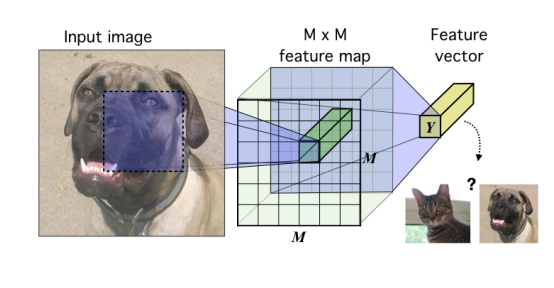
\includegraphics[width=\textwidth, height=5cm, natwidth=277, natheight=144]{Mal/deepinfo1.jpg}
  \caption{Базова модель кодера в контексті саних зображень.}
  \label{fig:deepinfo1}
\end{figure}

Подібно до принципу оптимізації infomax, можна стверджувати, що кодер повинен навчатися відповідно до таких критеріїв:

\begin{enumerate}
	\item максимізація взаємної інформації; 
	\item статистичні обмеження. 
\end{enumerate}


Максимізація взаємної інформації полягає в тому, що необхідно знайти набір параметрів $\psi$, таких, щоб взаємна інформація $L(X; E_{\psi} (X))$ була максимальною. Залежно від кінцевої цілі, ця максимізація може бути здійснена за повним входом $X$, або деякою структурованою або «локальною» підмножиною.

В той час як статистичні обмеження відповідають за те, що залежно від кінцевої мети для подання, граничні $\mathbb{U}_{\psi, \mathbb{P}}$ повинні відповідати апріорному розподілу ймовірності $\mathbb{V}$. Грубо кажучи, це може бути використано для заохочення вихідних даних кодера до бажаних характеристик (наприклад, незалежності).

Формулювання цих двох цілей називається Deep InfoMax (DIM) [4].

\subsubsection{Оцінка та максимізація взаємної інформації}

Основні рамки максимізації взаємної інформації представлені на рис. \ref{fig:deepinfo2}. 

\vspace{1em}

\begin{figure}[h]
  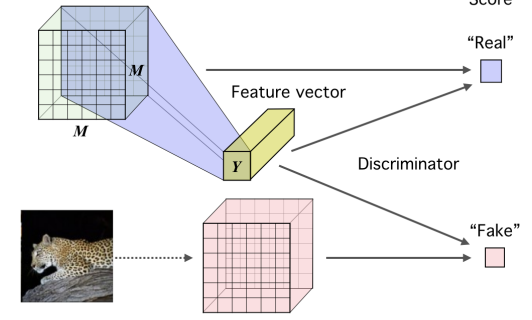
\includegraphics[width=\textwidth, height=5cm, natwidth=266, natheight=160]{Mal/deepinfo2.jpg}
  \caption{Deep InfoMax (DIM) з глобальною MI(X; Y) ціллю.}
  \label{fig:deepinfo2}
\end{figure}

Підхід слідує взаємній інформаційній нейронній оцінці (MINE), яка оцінює взаємну інформацію шляхом підготовки класифікатора для розрізнення зразків, що надходять із спільного розподілу $\mathbb{J}$ та відособленого розподілу $\mathbb{M}$ випадкових величин $X$ та $Y$. MINE використовує нижню межу для спільної інформації MI (від англійського mutual information) на основі представлення Донскер$-$Варадхана (DV) KL-дивергенції:

\begin{equation}\label{eq:dv}
L(X; Y) := D_{KL}(\mathbb{J}||\mathbb{M}) \ge \hat{L}_{\omega}^{DV}(X;Y):=\mathbb{E}_{\mathbb{F}}|T_{\omega}(x,y)| - \log{\mathbb{E}_{\mathbb{M}}[e^{T_{\omega}(x,y)}}],
\end{equation}

\noindent де $T_{\omega}: X \times Y \rightarrow \mathbb{R}$ функція дискримінатора, змодельована нейронною\newline 
\hspace*{15pt}мережею з параметрами $\omega$.

\vspace{1.5em}

На найвищому рівні оптимізується $\mathbb{E_{\psi}}$ одночасно оцінюючи та максимізуючи $L(X, E_{\psi}(X))$,

\begin{equation}\label{eq:e_psi_opt}
(\hat{\omega}, \hat{\psi})_{G} = \underset{\omega,\psi}{\arg\max}\hat{L}_{\omega}(X;E_{\psi}(X)),
\end{equation}

\vspace{1.5em}

\noindent де нижній індекс $G$ позначає «глобальний». 

Однак існують деякі важливі відмінності, які відрізняють цей підхід від MINE. По-перше, оскільки кодер і оцінювач взаємної інформації оптимізують одну і ту ж мету і вимагають подібних обчислень, ми ділимо шари між цими функціями, так що: 

\begin{equation}\label{eq:hz}
	E_{\psi} = f_{\psi} \circ C_{\psi} \, \text{та} \, T_{\psi, \omega} = D \circ g \circ (C_{\psi}, E_{\psi}), 
\end{equation}

\noindent де $g$ - функція, яка поєднує вихідні дані кодера з нижчим шаром.

\vspace{1.5em}

По-друге, враховуючи зацікавленність в максимальному збільшенні MI і не турбуючись його точним значенням, можна покластися на розбіжності, не пов’язані з KL, які можуть запропонувати вигідні компроміси. Наприклад, можна визначити оцінювач МІ Дженсена-Шеннона:

\begin{eqnarray}\label{eq:mi}
%\begin{aligned}
\hat{L}_{\omega, \psi}^{(infoNCE)}(X;E_{\psi}(X)) := \\ := \mathbb{E_{P}}\left[T_{\psi,\omega}(x, E_{\psi}(x)) - \mathbb{E_{\tilde{P}}}\left[\log{\sum_{x'}{e^{T_{\psi, \omega}(x',E_{\psi}(x))}}}\right]\right],
%\end{aligned}
\end{eqnarray}

\noindent де $x$ $-$ вхідний зразок, \newline
\hspace*{15pt} $x'$ $-$ вхід, відібраний з $\tilde{\mathbb{P}} = \mathbb{P}$, \newline
\hspace*{15pt} $sp(z) = \log{(1 + e^{z})}$ $-$ функція softplus. 

\vspace{1.5em}

Подібний оцінювач з'явився у контексті мінімізації сумарної кореляції, і це становить знайому двійкову перехресну ентропію. Це добре розуміється з точки зору оптимізації нейронних мереж, що на практиці такий підхід працює краще (наприклад, є стабільнішим), ніж ціль на основі DV. Інтуїтивно оцінювач, що базується на Йенсена-Шеннона, повинен поводитись подібно до оцінювача, що базується на DV в рівнянні. \ref{eq:mi}, оскільки обидва діють як класифікатори, цілі яких максимізують очікуване $log$-співвідношення з'єднання над добутком маржиналів.

Оцінка контрастності шуму (Noise-Contrastive Estimation) також може використовуватися з DIM шляхом максимізації:

\begin{equation}\label{eq:dim}
\hat{L}_{\omega,\psi}^{infoNCE}(X; E_{\psi}(X)) := \mathbb{E_{P}}\left[T_{\psi,\omega}(x, E_{\psi}) - \mathbb{E_{\tilde{P}}}\left[\log{\sum_{x'}{e^{T_{\psi, \omega}(x', E_{\psi}(x))}}}\right]\right].
\end{equation}

\vspace{1.5em}

Для DIM ключовою різницею між формулюваннями DV, JSD та infoNCE є те, чи з'являється очікування над $\mathbb{P / \tilde{P}}$ всередині $log$ або поза ним. Насправді ціль, що базується на JSD, відображає оригінальну формулювання NCE, яка формулює ненормалізовану оцінку щільності як двійкову класифікацію між розподілом даних та розподілом шуму. DIM встановлює розподіл шуму на добуток граничних значень на $X / Y$, а розподіл даних $-$ на справжнє з'єднання. Формулювання infoNCE слідує версії NCE на основі softmax, подібній до тих, що використовуються у спільноті моделювання мов і яка має міцні зв'язки з бінарною перехресною ентропією в контексті поріввняльного навчання. На практиці реалізації ці оцінювачи здаються досить схожими і можуть повторно використовувати більшість того самого коду. Дослідження JSD та infoNCE у експериментах дозволяє виявити, що використання infoNCE часто перевершує JSD у подальших завданнях, хоча цей ефект зменшується із більш складними даними. Однак для того, щоб infoNCE та DV вимагали великої кількості негативних зразків (зразки з $\mathbb{\tilde{P}}$), вони повинні бути конкурентоспроможними.

\subsubsection{Максимізація локальної спільної інформації}

Критерій в рівнянні \ref{eq:e_psi_opt}  можна використовувати для максимізації MI між входом і виходом, але в кінцевому рахунку це може бути небажаним залежно від завдання. Наприклад, тривіальний шум на рівні пікселів марний для класифікації зображень, тому подання може не отримати вигоди від кодування цієї інформації (наприклад, при навчанні з нульовим знімком, навчанні передачі тощо). Для того, щоб отримати представлення, більш придатне для класифікації, можна замість цього максимізувати середній MI між представленням високого рівня та локальними плямами зображення. Оскільки одному і тому ж представництву рекомендується мати високий MI з усіма патчами. це надає перевагу кодуванню аспектів даних, які спільно використовуються між патчами.

Припустимо, що вектор ознак має обмежену ємність (кількість одиниць та діапазон) і припустимо, що кодер не підтримує нескінченні вихідні конфігурації. Для максимізації MI між усім входом і поданням, кодер може вибрати який тип інформації на вході передається через кодер, наприклад, шум, характерний для локальних латок або пікселів. Однак, якщо кодер передає інформацію, характерну лише для деяких частин вводу, це не збільшує МІ з будь-якими іншими патчами, які не містять згаданого шуму. Це спонукає кодер віддавати перевагу інформації, яка передається у вхідних даних [4].

DIM-фреймворк представлено на рис. \ref{fig:deepinfo3}. 

\vspace{1em}

\begin{figure}[h]
  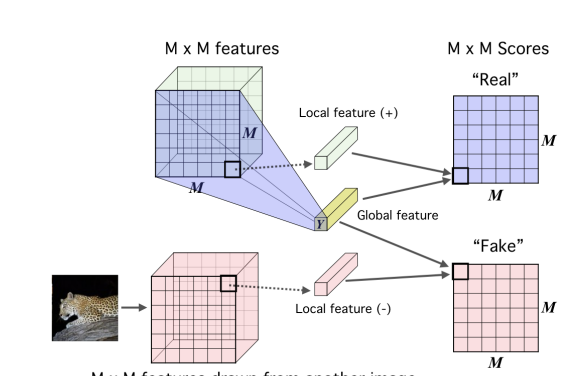
\includegraphics[width=\textwidth, height=5cm, natwidth=291, natheight=188]{Mal/deepinfo3.jpg}
  \caption{Максимізація взаємної інформації між локальними та глобальними характеристиками.}
  \label{fig:deepinfo3}
\end{figure}

Спочатку потрібно закодувати вхідні дані до карти об’єктів, $C_{\psi} = \left\{ C_{\psi}^{(i)} \right\}_{i=1}^{M \times M}$, що відображає корисну структуру в даних, індексовану в цьому випадку $i$. Далі, можна узагальнити цю локальну карту об’єктів у загальну характеристику: $E_{\psi} = f_{\psi} \circ C_{\psi}(x)$. Потім необхідно визначити оцінювач MI на глобальних та локальних парах, максимізуючи середню оцінку MI:

\begin{equation}\label{eq:max_mi}
(\hat{\omega}, \hat{\psi})_{L} = \underset{\omega,\psi}{\arg\max}\frac{1}{M^{2}}\sum_{i=1}^{M^{2}}\hat{L}_{\omega, \psi}(C_{\psi}^{(i)}(X); E_{\psi}(X)).
\end{equation}

\vspace{1.5em}

\subsubsection{Відповідність представлень апріорному розподілу}

Абсолютна величина інформації є лише однією бажаною властивістю уявлення. Залежно від програми хороші уявлення можуть бути компактними, незалежними, розплутаними або незалежно керованими. DIM накладає статистичні обмеження на вивчені уявлення, неявно навчаючи кодер так, щоб образ міри $\mathbb{U_{\psi, P}}$ збігався з попереднім $\mathbb{V}$. Це робиться шляхом навчання дискримінатора, $D_{\phi} : Y \rightarrow \mathbb{R}$, для оцінки розбіжності, $D(\mathbb{V} || \mathbb{U_{\psi, P}})$. Після чого тренуємо кодер для мінімізації оцінки:

\begin{eqnarray}\label{eq:div}
%\begin{aligned}
(\hat{\omega}, \hat{\psi})_{P} \underset{\psi}{\arg\min}\,\underset{\phi}{\arg\max}\hat{D}_{\phi}(\mathbb{V}||\mathbb{U_{\psi,P}}) = \mathbb{E_{V}}[\log{D_{\phi}(y)}] + \\ + \mathbb{E_{P}}[\log{(1-D_{\phi}(E_{\psi}(x)))}].
%\end{aligned}
\end{eqnarray}

\vspace{1.5em}

Цей підхід подібний до того, що робиться в змагальних автокодерах, але без генератора. Він також схожий на шум як цілі, але тренує кодер, щоб він неявно відповідав шуму, а не використовував апріорні вибірки шуму як цілі.

Всі три цілі: глобальна та локальна максимізація МІ та попереднє узгодження можуть бути використані разом. І, таким чином, можна отримати критерій Deep InfoMax (DIM):

\begin{eqnarray}\label{eq:deepinfomax}
%\begin{aligned}
\underset{\omega_{1},\omega_{2},\psi}{\arg\max}(\alpha \hat{L}_{\omega_{1},\psi}(X; E_{\psi}(X)) + \frac{\beta}{M^{2}}\sum_{i=1}^{M^{2}}{\hat{L}_{\omega_{2}, \psi}(X^{(i)}; E_{\psi}(X)))} + \\
+ \underset{\psi}{\arg\min}\,\underset{\phi}{\arg\max}\gamma\hat{D}_{\phi}(\mathbb{V}||\mathbb{U_{\psi,P}}),
%\end{aligned}
\end{eqnarray}

\noindent де $\omega_{1}$ та $\omega_{2}$ $-$ параметри дискримінатора відповідно до глобальних \newline
\hspace*{15pt}та локальних цілей, \newline
\hspace*{15pt}$\alpha$, $\beta$ та $\gamma$ $-$ гіперпараметри.

\vspace{1.5em}

\subsection{Momentum Contrast}

Порівняльне навчання та його останні розробки можна розглядати як навчання кодеру для завдання пошуку у словнику.

Розглянемо закодований запит $q$ та набір закодованих зразків $\{k_{0}, k_{1}, k_{2}, \dots\}$, які є ключами словника. Припустимо, що у словнику є один ключ (позначений як $k_{+}$), який відповідає $q$. Контрастивна втрата $-$ це функція, значення якої є низьким, коли $q$ подібне до його позитивного ключа $k_{+}$ та відрізняється від усіх інших ключів (вважається негативним ключем для $q$). Можна перевизначити функцію InfoNCE:

\begin{equation}\label{eq:infonce_simple}
L_{q} = -\log{\frac{exp(q \cdot k_{+}/\tau)}{\sum_{i=0}^{K}{exp(q \cdot k_{i}/\tau)}}},
\end{equation}

\vspace{1.5em}

\noindent де $\tau$ гіперпараметр. 

Сума складається з однієї позитивної та $K$ негативних екземплярів. Інтуїтивно, ця втрата є логаріфмічною втратою класифікатора на основі $(K + 1)$ softmax, який намагається класифікувати $q$ як $k_{+}$. Функції контрастивних збитків можуть також базуватися на інших формах, таких як маржові збитки та варіанти збитків NSE.

Контрастивна втрата служить неконтрольованою цільовою функцією для навчання мереж кодера, що представляють запити та ключі. Загалом, подання запиту має значення $q = f_{q} (x^{q})$, де $f_{q}$ - це мережа кодера, а $x^{q}$ - зразок запиту (так само, $k = f_{k} (x^{k})$). Їх екземпляри залежать від конкретного попередньогозавдання. Вхідними даними $x^{q}$ та $x^{k}$ можуть бути зображення, патчі або контекст, що складається з набору патчів. Мережі $f_{q}$ і $f_{k}$ можуть бути ідентичними, частково спільними або різними.

З вищенаведеної точки зору, порівняльне навчання $-$ це спосіб побудови дискретного словника на безперервних вхідних даних, таких як зображення. Словник є динамічним у тому сенсі, що ключі вибираються випадково, а кодер ключів розвивається під час навчання. Гіпотеза полягає в тому, що хорошим можливостям можна навчитися за допомогою великого словника, який охоплює багатий набір негативних зразків, тоді як кодер ключів словника зберігається якомога послідовнішим, незважаючи на його розвиток. Виходячи з цього можна описати алгорим Momentum Contrast.

В основі цього підходу лежить підтримка словника як черги зразків даних. Це дозволяє нам повторно використовувати закодовані ключі з безпосередніх попередніх міні-пакетів. Введення черги відокремлює розмір словника від розміру міні-партії. Розмір словника може бути набагато більшим, ніж типовий розмір міні-партії, і може бути гнучко та незалежно встановлений як гіперпараметр.

Зразки у словнику поступово замінюються. Поточна міні-партія потрапляє до словника, а найстаріша міні-партія в черзі вилучається. Словник завжди представляє вибіркову підмножину всіх даних, тоді як додаткові обчислення ведення цього словника є керованими. Більше того, видалення найстарішої міні-партії може бути корисним, оскільки її закодовані ключі є найбільш застарілими і, отже, найменш відповідають найновішим.

Використання черги може зробити словник великим, але це також робить важким оновлення кодера ключа шляхом зворотного розповсюдження (градієнт повинен поширюватися на всі зразки в черзі). Наївним рішенням є копіювання кодера ключа $f_{k}$ з кодера запиту $f_{q}$, ігноруючи цей градієнт. Але це рішення дає погані результати в експериментах. Припустимо, що такий збій спричинений швидко мінливим кодером, який зменшує узгодженість ключових подань. Пропонується оновити імпульс для вирішення цієї проблеми.

Формально, позначаючи параметри $f_{k}$ як $\theta_{k}$, а параметри $f_{q}$ як $\theta_{q}$, ми оновлюємо $\theta_{k}$ за допомогою:

\begin{equation}\label{eq:theta_opt}
\theta_{k} \leftarrow m\theta_{k} + (1 - m)\theta_{q}.
\end{equation}

\vspace{1.5em}

Тут $m \in [0, 1)$ $-$ коефіцієнт імпульсу. Тільки параметри $\theta_{q}$ оновлюються шляхом зворотного розповсюдження. Оновлення імпульсу в рівнянні \ref{eq:theta_opt} змушує $\theta_{k}$ еволюціонувати більш плавно, ніж $\theta_{q}$. Як результат, хоча ключі в черзі кодуються різними кодерами (в різних міні-партіях), різниця між цими кодерами може бути невеликою. В експериментах порівняно великий імпульс (наприклад, m = 0,999, за замовчуванням) працює набагато краще, ніж менший показник (наприклад, m = 0,9), що дозволяє припустити, що кодер ключів, який повільно розвивається, є стрижнем для використання черги.

MoCo $-$ загальний механізм використання контрастивних втрат. Ми порівнюємо це з двома існуючими загальними механізмами на рис \ref{fig:momentum1}. Вони мають різні властивості щодо розміру та послідовності словника.

\vspace{1em}

\begin{figure}[h]
  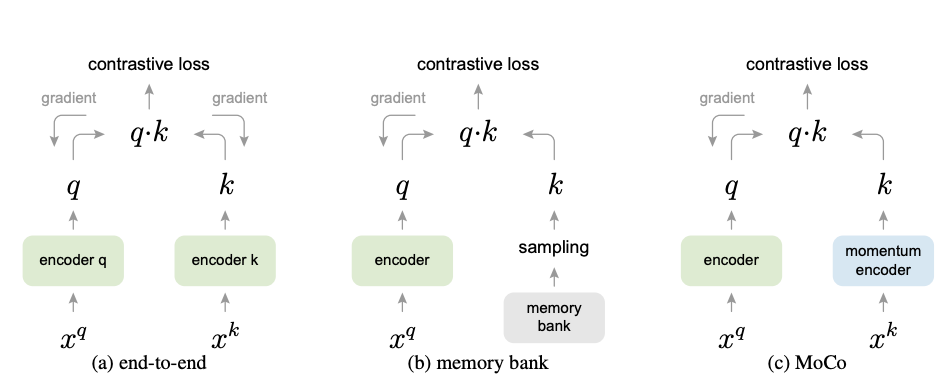
\includegraphics[width=\textwidth, height=5cm, natwidth=474, natheight=193]{Mal/momentum1.jpg}
  \caption{Концептуальне порівняння трьох контрастивних механізмів втрат.}
  \label{fig:momentum1}
\end{figure}

Оновлення end-to-end шляхом зворотного розповсюдження є природним механізмом. Він використовує зразки в поточній міні-партії як словник, тому ключі послідовно кодуються (тим самим набором параметрів кодера). Але розмір словника поєднується з міні-пакетним розміром, обмеженим обсягом пам'яті графічного процесора. Це також кидається виклик великій міні-пакетній оптимізації. Деякі останні методи засновані на завданнях підтексту, керованих місцевими позиціями, де розмір словника може бути збільшений на кілька позицій. Але для цих завдань-претекстів можуть знадобитися спеціальні мережеві конструкції, такі як патчіфікація вводу або налаштування сприйнятливого розміру поля, що може ускладнити перенесення цих мереж на подальші завдання [5].

Іншим механізмом є підхід банк пам'яті (memory bank). Банк пам'яті складається з подань усіх зразків у наборі даних. Словник для кожної міні-партії вибірково вибирається з банку пам'яті без зворотного розповсюдження, тому він може підтримувати великий розмір словника. Однак представлення вибірки в банку пам'яті було оновлено, коли її востаннє бачили, тому вибіркові ключі, по суті, стосуються кодерів на декількох різних етапах протягом усієї минулої епохи і, отже, менш послідовні. Оновлення імпульсу приймається на банку пам'яті. Її імпульс оновлення подається на поданнях того самого зразка, а не на кодері. Це оновлення імпульсу не має значення для нашого методу, оскільки MoCo не відстежує кожен зразок. Більше того, наш метод є більш ефективним в пам’яті, і його можна навчити на мільярдних даних, що може бути важко для банку пам'яті [5].

Порівняльне навчання може працювати з різними попередніми задачами.

Можна розглянути запит і ключ як позитивну пару, якщо вони походять з одного зображення, а в іншому $-$ як негативну пару вибірки. Візьмемо два випадкові «види» одного і того ж зображення під час випадкового збільшення даних, щоб сформувати позитивну пару. Запити та ключі кодуються відповідними кодерами $f_{q}$ та $f_{k}$. Кодером може бути будь-яка згорткова нейронна мережа.

Алгоритм Momentum Contrast для попередньої задачі можна реалізовувати по-різному. Наприклад: адаптувати нейронну мережу ResNet як кодер, чий останній повністю підключений шар (після загального середнього об'єднання) має вихід з фіксованим розміром (128-D). Цей вихідний вектор нормується за його L2-нормою. Це представлення запиту або ключа. Після чого потрібно обрати значення для аргументу $\tau$ з \ref{eq:infonce_simple}. Далі наведено параметр збільшення даних: обрізання $224 \times 224$ пікселів береться із зображення випадкового розміру, а потім піддається випадковому коливанню кольорів, випадковому горизонтальному перевертанню та випадковому перетворенню шкал сірого.

Обидва кодери $f_{q}$ і $f_{k}$ використовують пакетну нормалізацію (Batch Normalization, BN), як у стандартному ResNet. Можна показати, що використання BN заважає моделі засвоїти хороші уявлення.

Цю проблему можливо вирішити за допомогою тасування BN. Можна тренувати модель з декількома графічними процесорами та виконуввати BN на зразках незалежно для кожного графічного процесора (як це робиться у звичайній практиці). Для кодера ключів $f_{k}$ перемішується порядок зразків у поточній міні-партії перед розподілом між графічними процесорами (і перемішується назад після кодування). Порядок вибірки міні-партії для кодера запиту $f_{q}$ не змінюється. Це гарантує, що статистична інформація про партії, яка використовується для обчислення запиту, та її позитивний ключ надходять із двох різних підмножин. Це ефективно вирішує проблему дозволяє тренуванню принести користь від BN.

Використання перемішаного BN може стати у нагоді також у end-to-end оновленні. Це не має значення для банку пам'яті, який не страждає від цієї проблеми, оскільки позитивні ключі були від різних міні-пакетів у минулому.

\subsection{Висновки за розділом}

Порівняльне навчання $-$ це техніка машинного навчання, яка використовується для вивчення загальних особливостей набору даних без міток, навчаючи моделі, які точки даних подібні чи різні [6].

В результаті огляду літературних джерел для аналізу були обрані алгоритми Deep InfoMax (DIM) та Momentum Contrast (MoCo).
